\begin{figure}[h]
\centering
\fbox{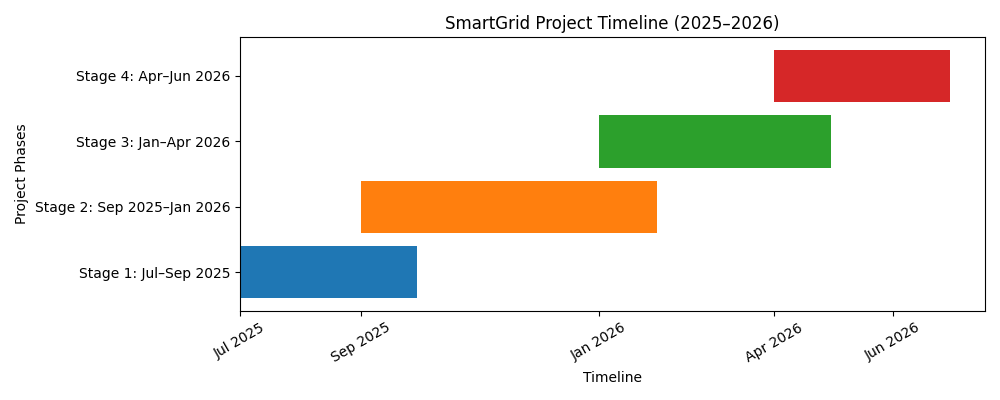
\includegraphics[width=0.9\textwidth]{chart.png}}
\caption{Project timeline }
\label{fig:Gantt Chart}
\end{figure}


\noindent
The project timeline is structured into four overlapping stages spanning July 2025 to June 2026, reflecting the iterative and incremental development approach adopted in this work. 

Stage 1 (July--September 2025) focuses on problem formulation, dataset preparation, and baseline experimentation. Stage 2 (September 2025--January 2026) involves feature engineering and prototype development, including the initial implementation of the anomaly detection framework. Stage 3 (January--April 2026) covers model refinement, system integration, and full evaluation across different configurations. Finally, Stage 4 (April--June 2026) is dedicated to documentation, system packaging, and preparation for final presentation and defense.

The overlap between stages shows parallel progress, where findings from later phases fed back into earlier design decisions and led to ongoing changes throughout the project.